\section{数学分析}
\subsection{反三角函数的化解}  
\begin{theorem}[反三角函数化解]
     \begin{equation}
        \arccos \frac{1}{x}=\operatorname{arcsec} x 
     \end{equation}
\end{theorem} 


\begin{proof}

\begin{minipage}[b]{0.4\linewidth}
    \begin{align*}
        &\mathtext{欲证:}  \arccos \frac{1}{x}=\operatorname{arcsec} x \\
        &\mathtext{即证:}  \cos \left[\arccos \frac{1}{x}\right]=\cos [\operatorname{arcsec} x] \\
        &\mathtext{即证:}  \frac{1}{x}=\cos [\operatorname{arcsec} x] \\
        &\mathtext{另有}  \arctan x+\arctan \frac{1}{x}=\frac{\pi}{2} \Rightarrow x \in\left(0, \frac{\pi}{2}\right) 
    \end{align*}
    \end{minipage}
    \hfill
    % 原来使用图片插入的方式
    % \begin{minipage}[b]{0.4\linewidth}
    %     \ctikzfig{Chapter/TikZ/trangle}
    % \end{minipage}
    \begin{minipage}[t]{0.4\linewidth}
        \begin{tikzpicture}[scale=2.5]
            \draw[fill=Blue!40, draw=Blue] %
                (0, 0) node[above right = 3pt and 2.5em] {$\alpha$} %
                --(2, 0) node[below left = 3pt and 6em] {$1$} %
                --(2, 1.2) node[below right = 4em and 3pt] {$x$}%
                --(0, 0);
            \draw (.4, 0) arc (0:31:.4);
        \end{tikzpicture}
    \end{minipage}
\end{proof}


\subsection{和差化积公式}
\begin{theorem}[和差化积公式]
    \noindent{一些记号:余$\Longrightarrow$鱼(渔)}
    \begin{align}{}
        &\cos(\alpha)+\cos(\beta)=2\cos(\frac{\alpha+\beta}{2})\cos(\frac{\alpha-\beta}{2})&&\hspace*{10em}\mathtext{鱼 + 鱼 = 2条鱼}\nonumber \\
        &\cos(\alpha)-\cos(\beta)=-2\sin(\frac{\alpha+\beta}{2})\sin(\frac{\alpha-\beta}{2})&&\hspace*{10em}\mathtext{鱼 - 鱼=没有鱼}\nonumber \\
        &\sin(\alpha)-\sin(\beta)=2\cos(\frac{\alpha+\beta}{2})\sin(\frac{\alpha-\beta}{2})&&\hspace*{10em}\mathtext{兄弟不和,渔翁得利}\nonumber \\
        &\sin(\alpha)+\sin(\beta)=2\sin(\frac{\alpha+\beta}{2})\cos(\frac{\alpha-\beta}{2})&&\hspace*{10em}\mathtext{兄弟相和,渔翁失利}
    \end{align}
\end{theorem}


\subsection{两个三角恒等式的证明}
\begin{theorem}[三角恒等式]
    \begin{flalign}
        &\sum_{k=1}^{n}{\sin(kx)}=\frac{\cos(n+\frac{1}{2})-\cos(\frac{x}{2})}{-2\sin(\frac{x}{2})}\nonumber\\
        &\sum_{k=1}^{n}{\cos(kx)}=\frac{\sin(n+\frac{1}{2})-\sin(\frac{x}{2})}{2\sin(\frac{x}{2})}
    \end{flalign}
\end{theorem}

\begin{proof}
\begin{align*}
    \sum_{k=1}^{n}{\sin(kx)}
    &=\frac{1}{\sin(\frac{x}{2})}[\sin(\frac{x}{2})\sin(x)+\sin(\frac{x}{2})\sin(2x)+\cdots+\sin(\frac{x}{2})\sin(nx)]\\
    &=\frac{1}{-2\sin(\frac{x}{2})}[[\cos(\frac{3x}{2})-\cos(\frac{x}{2})]+[\cos(\frac{5x}{2})-\cos(\frac{3x}{2})]+\cdots+[\cos(n+\frac{1}{2})x-\cos((n-\frac{1}{2})x)]]\\
    &=\frac{1}{-2\sin(\frac{x}{2})}[-\cos(\frac{x}{2})+\cos(n+\frac{1}{2})x]\\
    &=\frac{\cos(n+\frac{1}{2})x-\cos(\frac{x}{2})}{-2\sin(\frac{x}{2})}
\end{align*}
第二个式子证明时,同样只需要乘以$\frac{1}{\sin(\frac{x}{2})}$
\end{proof} 


\subsection{函数可微性的定义证明}

\begin{proof}
    $ y=\sqrt[\frac{3}{2}]{x}$可以写成:$\Delta y = A \Delta x + o(\Delta x)$
其中 $A=\sqrt[\frac{3}{2}]{x}=\frac{3}{2}x^{-\frac{1}{3}}$, 于是 $\Delta y$就具有如下的形式    


\begin{align}
\Delta y&= \sqrt[3]{(x+\Delta x)^2} -\sqrt[3]{x^2}\notag \Longrightarrow \mathtext{想办法凑出}\frac{2}{3}x^{-\frac{1}{3}}\mathtext{与}\Delta x\\
    &= \frac{x+\Delta x}{\sqrt[3]{x+\Delta x}}-\frac{x}{\sqrt[3]{x}}\notag\\
    &= \frac{2}{3}\frac{\Delta x}{\sqrt[3]{x}}+\overbrace{\textcolor{blue}{\frac{1}{3}\frac{\Delta x}{\sqrt[3]{x}}+(x+\Delta x)(\frac{1}{\sqrt[3]{x+\Delta x}}-\frac{1}{\sqrt[3]{x}})}}^{\mycircled{1}}\notag
\end{align}
我们把(1)中的蓝色部分记作\ding{172},  %% \ding{}不能用在数学环境里边
意味着我们只需要证明

\begin{align*}
    \lim_{\Delta x \rightarrow 0}\frac{\mycircled{1}}{\sqrt[3]{x}}=0
\end{align*}  
注:其实$\lim\limits_{\Delta x \rightarrow 0}{\frac{\frac{1}{\sqrt[3]{x+\Delta x}}-\frac{1}{\sqrt[3]{x}}}{\Delta x}}$就是求$\frac{1}{\sqrt[3]{x}} $的导数,
求出(2)的极限即可:

\begin{align}
    \lim_{\Delta x \rightarrow 0}\frac{\mycircled{1}}{\sqrt[3]{x}}
    &=\lim\limits_{\Delta x \rightarrow 0}{\frac{\frac{1}{\sqrt[3]{x+\Delta x}}-\frac{1}{\sqrt[3]{x}}}{\Delta x}}\notag\\
    &=\frac{x}{\Delta x}\left( \frac{\frac{-\Delta x}{x\left( x+\Delta x \right) }}{\frac{1}{\sqrt[3]{\left( x+\Delta x \right) ^2} }+\frac{1}{\sqrt[3]{\left( x\left( x+\Delta x \right)  \right) } }+\frac{1}{\sqrt[3]{x^2} }} \right) \notag\\
    &=\frac{-\frac{x}{x^2}}{\frac{1}{3\sqrt[3]{x^2} }}= -\frac{1}{3}x^{-\frac{1}{3}}\nonumber
\end{align}
总结:这里面主要就是用到因式分解公式: $a^3-b^3=\left( a-b \right)\left( a^2+ab+b^2 \right)  $
\end{proof}

\subsection{函数有界的理解}
在之前用函数在每一点有界推出这个函数有界,关键在函数所在的区间是{\sf 有限}的,不是无穷的。


\subsection{柯西审敛法中没有N的存在}

由于在运算过程中没有用到N的相关的性质,所以对于一切的N我们的推导过程都是成立的。如果你实在是要严格,你可以在最前边添加$\forall N> 0 ,\exists m_0 = p_0 ,\exists \varepsilon_0 = \frac{1}{2}$, 使得$10 > \varepsilon_0$


\subsection{二元函数中值定理的理解}
\begin{theorem}
    \begin{align}
        f(a+h, b+k) - f(a, b) = f_x(a+\theta h, b + \theta k)h + f_y(a+\theta h, b + \theta k)k, ~~~~&\theta \in (0, 1)
    \end{align}
\end{theorem}

对比一元函数的拉格朗日中值定理
\begin{align*}
    f(a+h) - f(a) = f_x(a+\theta h)h \qquad \theta \in (0, 1)
\end{align*}
实际上我们可以把二元的中值定理看作是两个一元函数中值定理的和,其实可以认为
就是 $x$ 和 $y$ 两个方向上的一元函数(偏导数 $f_x$ 和 $f_y$)

\subsection{Able判别法证明的一个反思}
已知有Abel判别法和Dirichlet判别法:
\begin{theorem}[Abel~Dirichlet判别法]
    \ensuremath{\displaystyle\sum_{n=1}^{\infty}{a_nb_n}}收敛,
    如果满足下列两个条件之一,  那么这个级数收敛。
    \begin{align*}
    & \num{1}\quad \{a_n\}\mathtext{单调有界,}~\sum_{i=1}^{\infty}{b_i}\mathtext{收敛} \\
    & \num{2}\quad \{a_n\}\mathtext{单调趋于0,}~\sum_{i=1}^{n}{b_i}\mathtext{有界} 
    \end{align*}
\end{theorem}


\noindent\textsf{错误的想法}\par
设$\{a_n\}$有上界A ,$\sum\limits_{}^{\infty}{b_n}$收敛于B

所以有$\sum\limits_{}^{\infty}{a_nb_n}<A \sum\limits_{}^{\infty}{b_n}=AB$

错因分析: $\{b_n\}$不一定是正项级数,不能用比较判别法

\noindent\textsf{正解}\par
\begin{align*}
    &\sum_{}^{\infty}{a_n(B_n-B_{n-1})} 
        = (a_1-a_2)B_1+\cdots+(a_n-a_{n-1})B_{n-1}+a_nB_n
\end{align*}
每一项都加绝对值有
\begin{align*}
    \mathrm{LHS}
    & =\bigg|\sum_{}^{\infty}{a_nb_n}\bigg|
      =\bigg|(a_1-a_2)B_1+\cdots+(a_n-a_{n-1})B_{n-1}+a_nB_n\bigg|
\end{align*}

设\ensuremath{\displaystyle |\sum_{\infty}{b_n}|=B} 于是有:
\begin{align*}
    |\sum_{\infty}{a_nb_n}|\ge A|(a_1-a_n)|+A|a_n|
    \ge (|a_1|+\cdots+ |a_n|)A 
    = 3\varepsilon A
\end{align*}


\newpage
\textcolor{orange}{\textbf{注:Abel判别法和Dirichlet判别法的联系如下}}

\begin{figure}[!htb]
    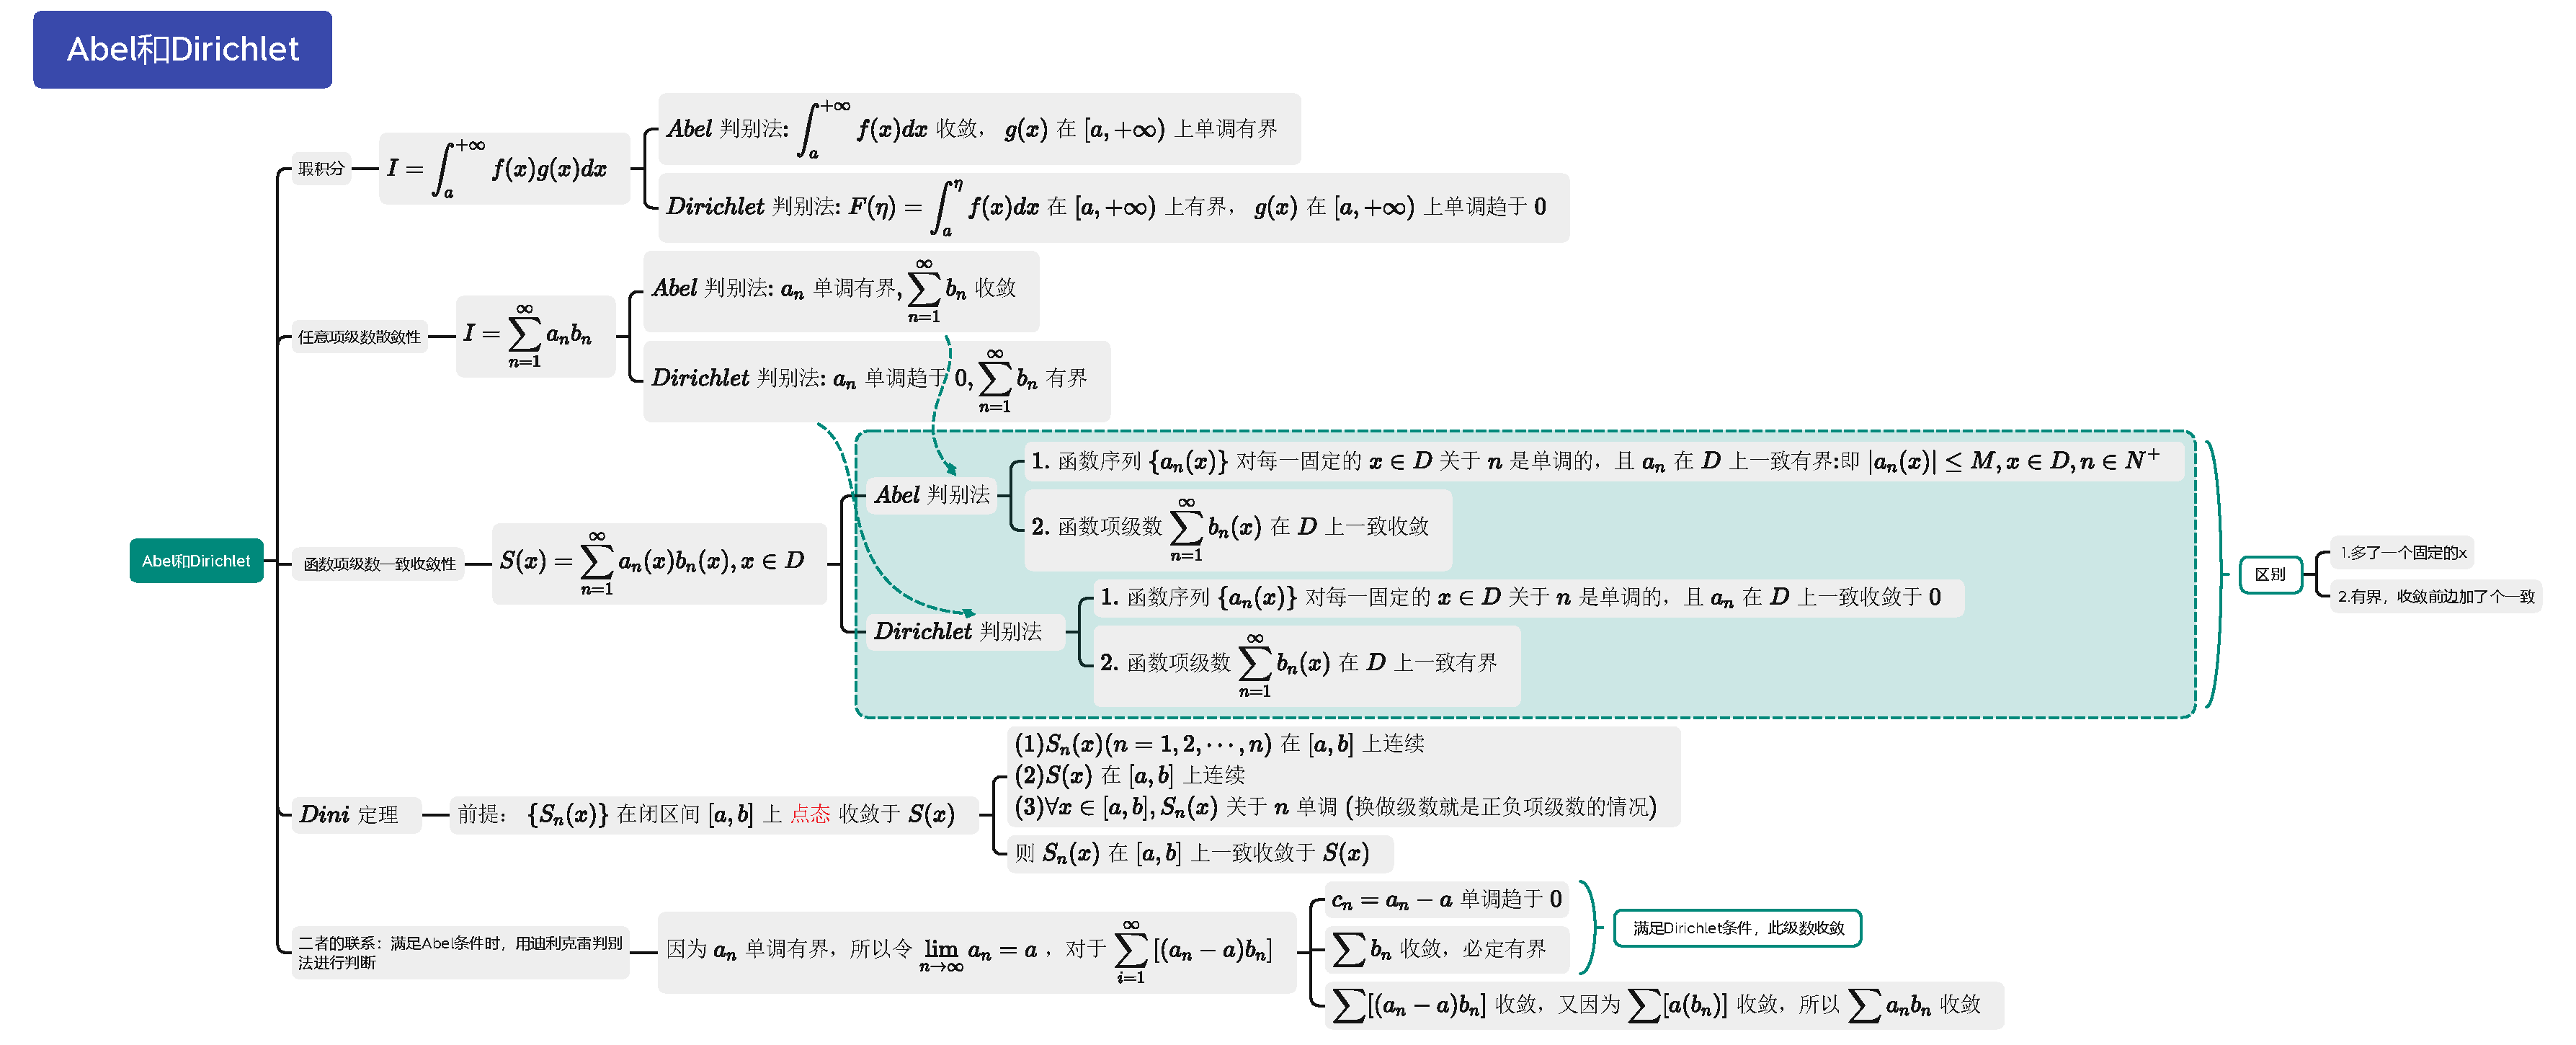
\includegraphics[scale=0.30]{Chapter/TikZ/Abel和Dirichlet.pdf}
    \label{Abel和Dirichlet}
    \caption{Abel和Dirichlet}
\end{figure}

那么判断级数的收敛性有什么作用呢?我们主要是应用它的如下性质:\par
\begin{figure}[!htb]
    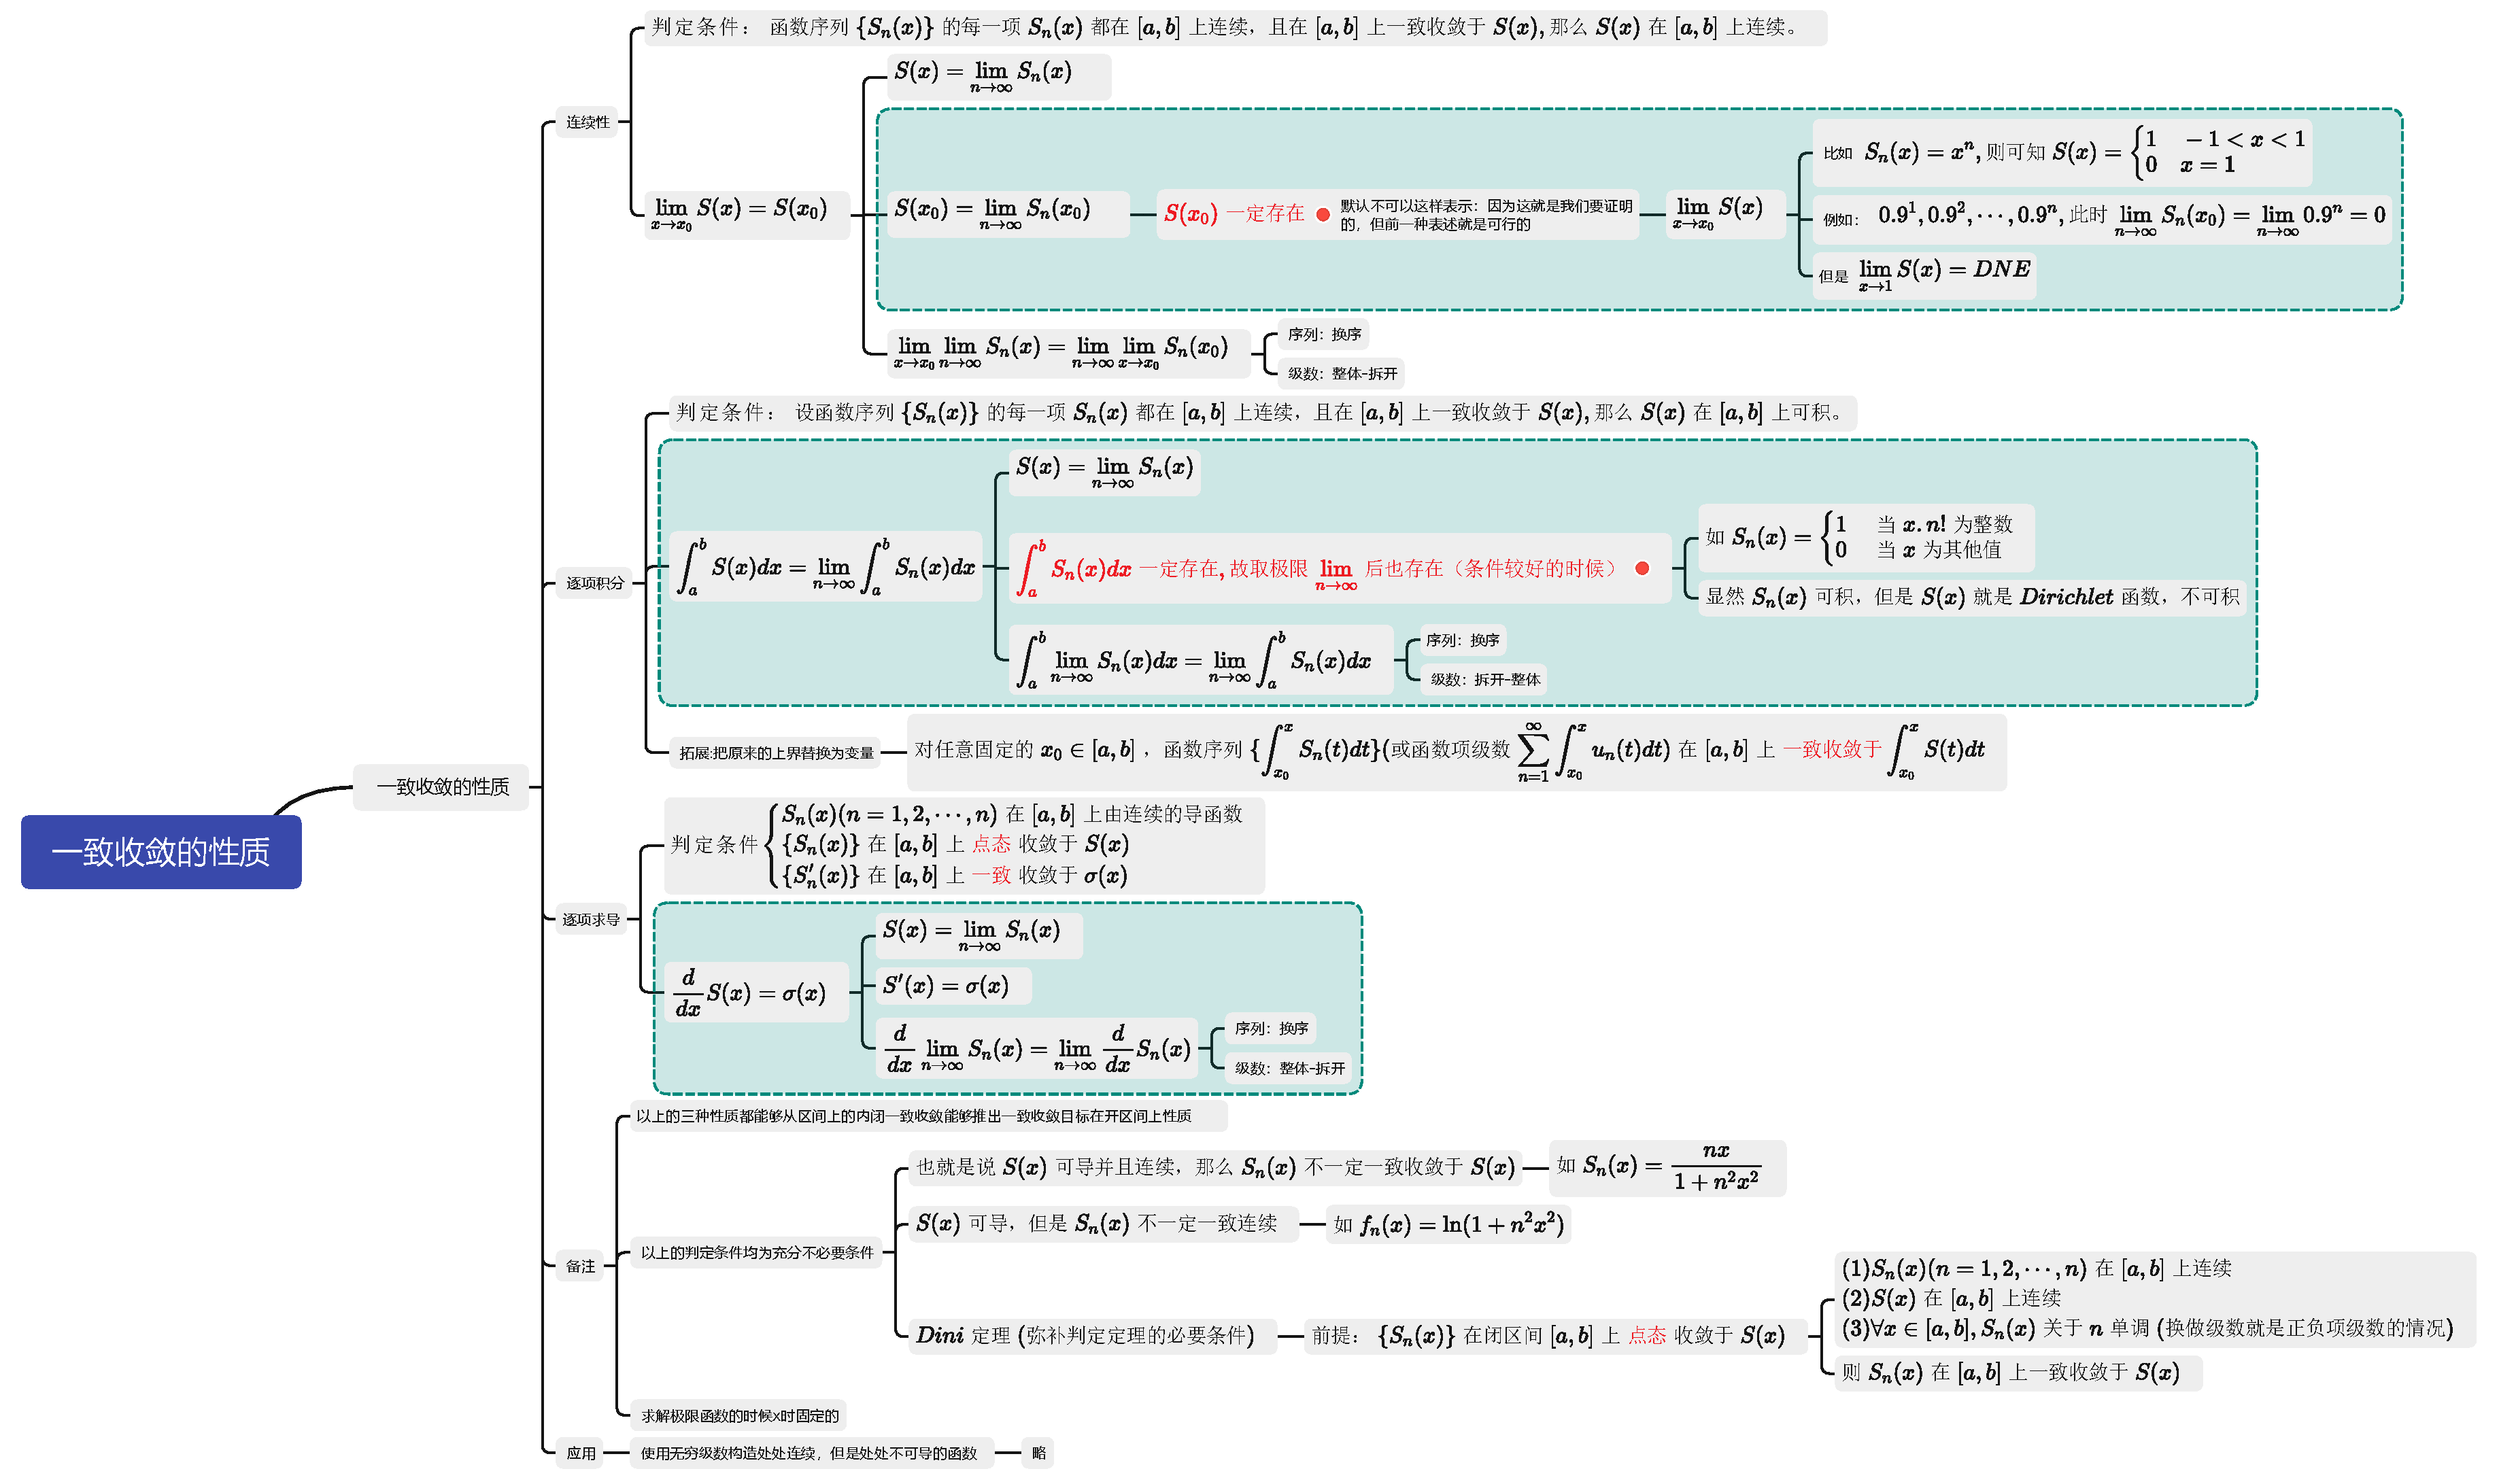
\includegraphics[scale=0.30]{Chapter/TikZ/一致收敛的性质.pdf}
    \label{一致收敛的性质}
    \caption{一致收敛的性质}
\end{figure}


\newpage
\section{极限}
\begin{definition}[极限定义]
    \textbf{\songti 函数极限的定义}\par
    $\forall \varepsilon>0, \exists \delta>0, 
    $当$|x-x_0|<\delta$时,~~ $\left|f(x)-f(x_0)\right|<\varepsilon$\par
    也就是说我的$f(x)$和$f(x_0)$可以无限接近,你要有多接近就有多接近,
    只要你给出接近的距离标准,比如 $0.1, 0.01, 0.001,\cdots$.我都有一个 $\delta$与之对应.\par
    
    \vspace*{2em}
    \textbf{\songti 它的逆否命题}\par
    $\forall \delta>0, \exists \varepsilon_0>0$
    当$\left|f(x)-f(x_0)\right|$时,~~$\left|x-x_0\right|>\delta$\par
    他的理解就恰恰和上边相反,你的$f(x)$和$f(x_0)$无法任意的接近,
    无论你的 $\delta$  取多么的小.$f(x)$和$f(x_0)$之间总会有一个无法跨越的最小距离 $\varepsilon_0$.
\end{definition}

\subsection{上,下极限}
上下极限的示意图

\begin{figure}[!htb]
    \centering
    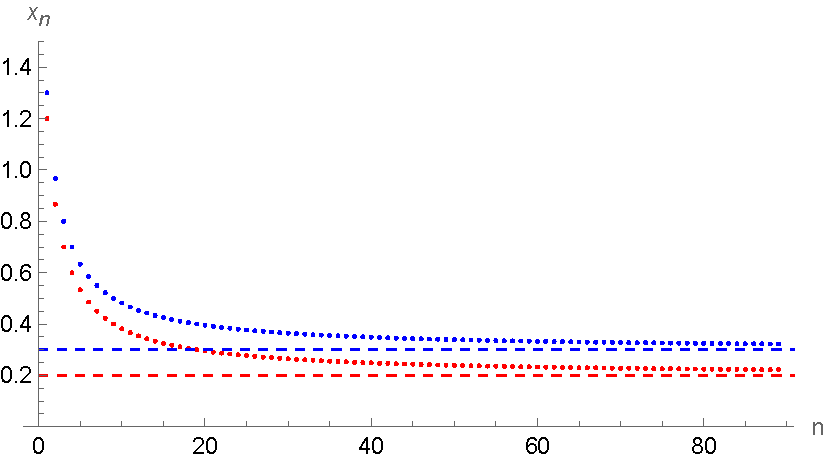
\includegraphics[scale=1]{Chapter/TikZ/上下极限散点图.pdf}
    \caption{上下极限散点图}   
\end{figure}



% 默认的行距是10pt
所有都$\ge$
$    
\begin{cases}
    \Longrightarrow \text{里边最小的都}\ge\\ 
    \Longrightarrow \text{里边的最大的也}\ge 
\end{cases}
\Longrightarrow x_n y_n \ge (H_1+\varepsilon)(H_2 + \varepsilon)
$


$\Longrightarrow \lim\limits_{n\to \infty}{x_ny_n} \ge \lim\limits_{n\to \infty}{(H_1+\varepsilon)(H_2 + \varepsilon)}$
$\Longrightarrow \lim\limits_{n\to \infty}{x_n y_n }\ge \lim\limits_{n\to \infty}{x_n}\cdot \lim_{n\to \infty}{y_n}$
问题在哪里?


